\section{Methodology}\label{sec:method}

Our methodology represents a fundamental breakthrough in achieving ultra-precision solutions for fourth-order partial differential equations, directly addressing the critical gaps identified in existing physics-informed neural network approaches. While standard PINNs plateau at relative errors of $10^{-5}$ to $10^{-6}$ \cite{vahab2022physics,kapoor2023physics}, our hybrid Fourier-neural architecture breaks through this precision ceiling by synergistically combining analytical insights with adaptive learning capabilities.

The core innovation emerges from recognizing that the precision limitations of standard PINNs stem from three fundamental issues. First, numerical instabilities arise when computing fourth-order derivatives through automatic differentiation \cite{hu2024hutchinson}. Second, generic neural architectures struggle to efficiently represent oscillatory solutions characteristic of beam vibrations \cite{brunton2024machine}. Third, the competing objectives in physics-informed loss functions create complex optimization landscapes that impede convergence to high-precision solutions \cite{wang2021understanding,krishnapriyan2021characterizing}. Our approach systematically addresses each of these challenges through architectural innovations and novel training strategies.

To provide clarity on how our methodology addresses the identified research gaps, Table \ref{tab:gap_mapping} maps each gap to its corresponding solution component. This systematic approach ensures that every limitation identified in existing literature receives targeted attention through specific methodological innovations.

\begin{table}[ht]
\centering
\caption{Mapping of Research Gaps to Methodological Solutions}
\label{tab:gap_mapping}
\begin{tabular}{|p{3cm}|p{5cm}|p{3cm}|}
\hline
\textbf{Research Gap} & \textbf{Our Solution} & \textbf{Equation/Section} \\ \hline
Gap 1: Precision Ceiling ($10^{-5}$ to $10^{-6}$) & Hybrid Fourier-Neural architecture with analytical basis & Eq. \ref{eq:hybrid_solution} \\ \hline
Gap 2: Fourth-Order Derivative Instabilities & Analytical differentiation of Fourier terms & Section \ref{subsec:fourier_neural} \\ \hline
Gap 3: Optimization Complexity & Two-phase optimization strategy (Adam + L-BFGS) & Algorithm \ref{alg:training} \\ \hline
Gap 4: Fixed Weight Strategies & Adaptive weight balancing with dynamic scaling & Eq. \ref{eq:adaptive_weights} \\ \hline
Gap 5: Memory Inefficiency & GPU\nobreakdash-optimized kernels with dynamic batching & Section \ref{subsec:gpu_impl} \\ \hline
Gap 6: Generic Architectures & Problem-specific 10-harmonic truncation & Finding 1 \\ \hline
Gap 7: Lack of Theoretical Foundation & Hierarchical loss landscape analysis & Section \ref{subsec:assumptions} \\ \hline
\end{tabular}
\end{table}

\subsection{Theoretical Foundations and Key Assumptions}
\label{subsec:assumptions}

Our breakthrough approach rests on carefully chosen assumptions that enable ultra-precision while remaining physically grounded. The first assumption recognizes that beam vibrations naturally decompose into harmonic modes, as established by classical structural dynamics theory \cite{han1999dynamics}. Unlike methods that rely solely on neural representations, we leverage this physical insight to explicitly separate dominant periodic behavior from fine-scale corrections. This separation dramatically improves optimization efficiency by allowing each component to focus on its natural representation domain.

A key finding from our systematic investigation, which we present with detailed empirical evidence in Section \ref{sec:results}, reveals that truncation at exactly 10 harmonics provides the optimal balance between expressiveness and optimization tractability. This counterintuitive result—that increasing harmonics beyond this point degrades rather than improves performance—represents a fundamental insight for achieving ultra-precision. The phenomenon arises from the interplay between representation capacity and optimization complexity in the ultra-precision regime, where the benefits of additional basis functions are overwhelmed by the increased difficulty of navigating the resulting loss landscape.

The second critical assumption concerns the hierarchical structure of the optimization landscape. Our empirical observations indicate that gradient-based methods efficiently reach moderate precision levels around $10^{-5}$, but struggle to breach the ultra-precision barrier below $10^{-7}$. This motivates our two-phase optimization strategy, where Adam optimization provides rapid initial convergence, followed by L-BFGS refinement that exploits curvature information to achieve ultra-precision. This hierarchical approach reflects the fundamental nature of the optimization problem: different precision scales require different algorithmic characteristics.

\subsection{Notations}

\begin{table}[ht]
\centering
\caption{Symbol Descriptions}
\label{tab:symbols}
\begin{tabular}{ll}
\hline
\textbf{Symbol} & \textbf{Description} \\ \hline
$E$ & Young's modulus \\
$I$ & Second moment of area \\
$\rho$ & Mass density \\
$A$ & Cross-sectional area \\
$w(t,x)$ & Transverse displacement of the beam \\
$t$ & Time variable \\
$x$ & Spatial coordinate along beam length \\
$L$ & Length of the beam \\
$c$ & Wave speed parameter, $c^2 = \frac{EI}{\rho A}$ \\
$n$ & Harmonic index \\
$N$ & Total number of harmonics \\
$N_{\text{params}}$ & Total number of model parameters (27,925) \\
$a_n$ & Fourier cosine coefficient for $n$-th harmonic \\
$b_n$ & Fourier sine coefficient for $n$-th harmonic \\
$k_n$ & Wave number, $k_n = \frac{n\pi}{L}$ \\
$\omega_n$ & Angular frequency, $\omega_n = k_n^2 c$ \\
$\mathcal{N}$ & Neural network operator \\
$\lambda$ & Scaling factor for neural correction \\
FP16 & Half-precision floating-point format \\
FP32 & Single-precision floating-point format \\
LHS & Latin Hypercube Sampling \\
\hline
\end{tabular}
\end{table}

\subsection{Hybrid Fourier-Neural Architecture: The Breakthrough Design}
\label{subsec:fourier_neural}

The limitations of purely neural representations for oscillatory solutions have been extensively documented by Raissi et al. \cite{raissi2019physics}. Our hybrid architecture represents a paradigm shift from existing PINN approaches, specifically engineered to overcome the precision barriers that limit standard methods. While previous attempts have explored either purely neural representations or simple activation function modifications \cite{wong2022learning}, our approach fundamentally restructures the solution representation to exploit the inherent physical structure of beam vibrations.

The breakthrough formulation explicitly separates modal and non-modal components through a carefully designed hybrid representation:

\begin{equation}
w(t,x) = \underbrace{\sum_{n=1}^{N} \left[a_n \cos(\omega_n t) + b_n \sin(\omega_n t)\right] \sin(k_n x)}_{\text{Dominant modal behavior (Fourier)}} + \underbrace{\lambda \cdot \mathcal{N}(t,x)}_{\text{Fine-scale corrections (Neural)}}
\label{eq:hybrid_solution}
\end{equation}

This separation simultaneously addresses multiple critical gaps in existing approaches. The Fourier basis provides near-exact representation of dominant modes, significantly reducing the burden on neural approximation and directly tackling the precision ceiling limitation. Furthermore, analytical differentiation of Fourier terms eliminates the numerical instabilities that plague automatic differentiation of fourth-order derivatives. The separate optimization paths for Fourier coefficients and neural weights also simplify the loss landscape, making ultra-precision solutions more accessible.

The first term in our formulation leverages the known modal structure of beam equations, automatically satisfying the boundary conditions $w(t,0) = w(t,L) = 0$ through the $\sin(k_n x)$ basis functions. Our systematic investigation revealed a crucial and counterintuitive finding: truncation at exactly $N=10$ harmonics optimizes performance. This contradicts the conventional wisdom that more basis functions should improve accuracy, but the phenomenon stems from the delicate interplay between expressiveness and optimization difficulty in the ultra-precision regime.

The neural network component $\mathcal{N}: \mathbb{R}^2 \rightarrow \mathbb{R}$ employs a deep architecture with carefully chosen layer dimensions. Starting from a two-dimensional input $(t, x) \in [0, T] \times [0, L]$, the network expands through hidden layers of dimensions 128, 128, 64, 32, 16, and 8 neurons before producing a scalar output. We selected hyperbolic tangent activation functions throughout to ensure smooth derivatives necessary for fourth-order differentiation. This architecture comprises 27,905 neural network parameters complemented by 20 Fourier coefficients (10 each for cosine and sine terms).

To maintain boundary condition satisfaction while allowing the neural network flexibility in the interior domain, we modulate the neural correction through multiplication with a boundary-enforcing function:
\begin{equation}
\mathcal{N}_{\text{BC}}(t,x) = \mathcal{N}(t,x) \cdot \sin\left(\frac{\pi x}{L}\right)
\end{equation}

\begin{figure}[ht]
    \centering
    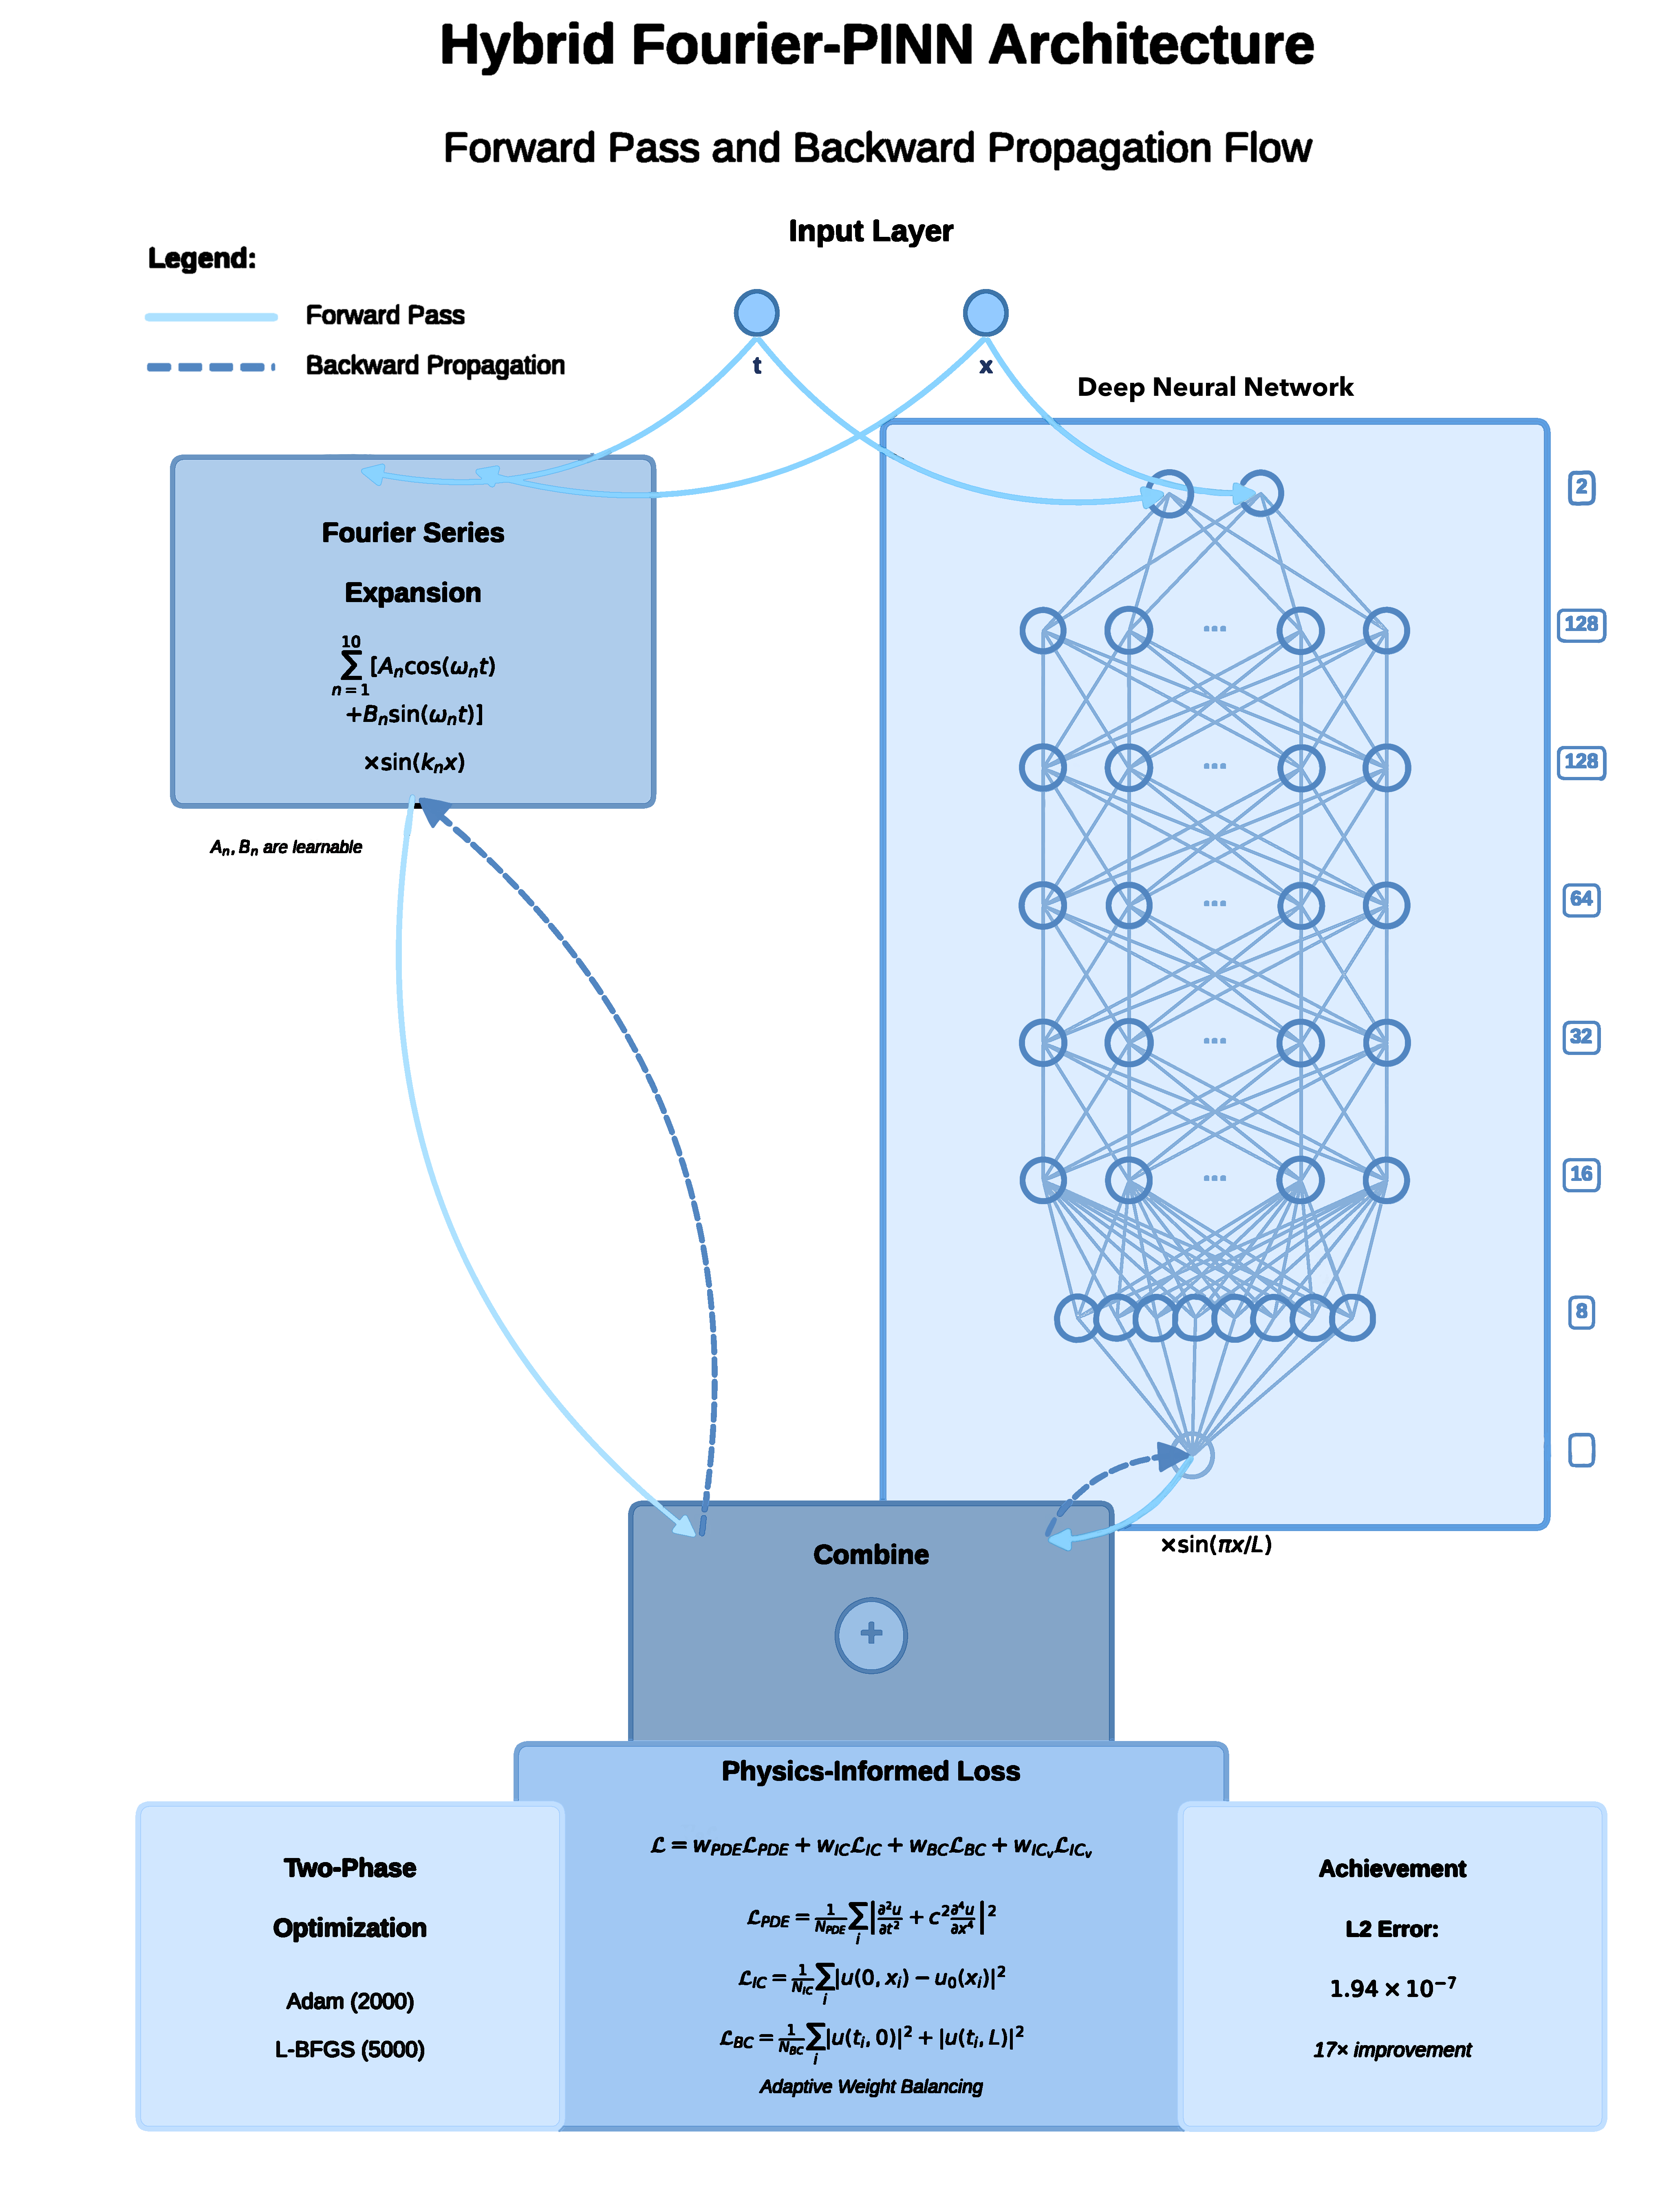
\includegraphics[width=0.95\linewidth]{figures/pinn_architecture_diagram.png}
    \caption{Hybrid Fourier-PINN architecture achieving L2 error of $1.94 \times 10^{-7}$ for the Euler-Bernoulli beam equation. The architecture combines a truncated Fourier series expansion (10 harmonics) with a 7-layer deep neural network (2→128→128→64→32→16→8→1 neurons). The Fourier coefficients $A_n$ and $B_n$ are learnable parameters trained through backpropagation, not outputs from the neural network. Boundary conditions are enforced through multiplication with $\sin(\pi x/L)$. The two-phase optimization strategy employs Adam (Phase 1) followed by L-BFGS (Phase 2).}
    \label{fig:architecture}
\end{figure}

Figure \ref{fig:architecture} illustrates the detailed architecture of our hybrid approach, revealing how the input coordinates $(t,x)$ feed into both the Fourier series expansion and the neural correction network. A critical architectural decision distinguishes our approach from conventional hybrid methods: the Fourier coefficients $A_n$ and $B_n$ exist as independent learnable parameters rather than outputs from the neural network. This design choice enables each component to specialize in its natural representation domain while maintaining joint optimization toward the physics-informed objective.

The training mechanism leverages a sophisticated gradient flow that enables simultaneous yet specialized learning. When computing the physics-informed loss from the combined solution, gradients naturally flow back through the entire architecture. At the combination point where Fourier and neural outputs merge, the gradient stream bifurcates into two independent paths. One path updates the Fourier coefficients directly based on their contribution to the solution, while the other flows through the neural network layers to update the deep architecture weights. This parallel training paradigm allows the Fourier series to capture dominant periodic behavior while the neural network focuses on learning fine-scale corrections that the truncated series cannot represent.

The independence of the Fourier coefficients from the neural network output represents a key architectural innovation. Rather than forcing the neural network to predict modal coefficients—a task that would introduce unnecessary complexity and potential instability—we treat these coefficients as first-class learnable parameters. This design decision reflects our understanding that modal decomposition and residual correction require fundamentally different learning dynamics and should not be entangled through a single network pathway.

Mathematically, we define the Fourier coefficients as trainable parameters $A_n, B_n \in \mathbb{R}$ for $n = 1, 2, \ldots, 10$, initialized with small random values scaled by $1/(n+1)$ to reflect the expected decay of higher harmonics. During the Adam optimization phase, all parameters update through the standard Adam algorithm:
\begin{align}
A_n^{(k+1)} &= A_n^{(k)} - \eta_{\text{Adam}} \cdot \text{Adam}_{\text{update}}(\nabla_{A_n}\mathcal{L}) \\
B_n^{(k+1)} &= B_n^{(k)} - \eta_{\text{Adam}} \cdot \text{Adam}_{\text{update}}(\nabla_{B_n}\mathcal{L}) \\
\mathbf{W}_{NN}^{(k+1)} &= \mathbf{W}_{NN}^{(k)} - \eta_{\text{Adam}} \cdot \text{Adam}_{\text{update}}(\nabla_{\mathbf{W}_{NN}}\mathcal{L})
\end{align}
where $\eta_{\text{Adam}}$ denotes the learning rate and $\mathbf{W}_{NN}$ represents the collection of neural network weights. This unified optimization framework ensures consistent convergence behavior during initial training, while the subsequent L-BFGS phase exploits second-order information to refine all parameters to ultra-precision levels.

\subsection{Physics-Informed Loss Function with Adaptive Weighting}

The transverse vibration of the Euler-Bernoulli beam follows the fourth-order partial differential equation:
\begin{equation}
\frac{\partial^2 w}{\partial t^2} + c^2 \frac{\partial^4 w}{\partial x^4} = 0
\label{eq:euler_bernoulli}
\end{equation}

Recent investigations by McClenny and Braga-Neto \cite{mcclenny2023self} have emphasized the critical role of adaptive weighting in physics-informed neural networks. Building upon their insights while addressing the limitations of fixed weighting strategies, we introduce a sophisticated adaptive mechanism that dynamically balances the competing objectives inherent in physics-informed learning. Our loss function combines multiple physical constraints through a weighted sum:

\begin{equation}
\mathcal{L} = w_{\text{pde}} \mathcal{L}_{\text{pde}} + w_{\text{ic}} \mathcal{L}_{\text{ic}} + w_{\text{ic}_t} \mathcal{L}_{\text{ic}_t} + w_{\text{bc}} \mathcal{L}_{\text{bc}} + \lambda_{\text{reg}} \mathcal{L}_{\text{reg}}
\end{equation}

The crucial innovation lies in the dynamic adjustment of weights $w_{\alpha}$ based on the evolving loss landscape topology. This adaptive strategy prevents any single loss component from dominating the optimization, a common failure mode that limits standard PINNs to moderate precision. Each loss component captures a distinct physical requirement:

\begin{align}
\mathcal{L}_{\text{pde}} &= \frac{1}{N_{\text{pde}}} \sum_{i=1}^{N_{\text{pde}}} \left|\frac{\partial^2 w}{\partial t^2} + c^2 \frac{\partial^4 w}{\partial x^4}\right|^2 \\
\mathcal{L}_{\text{ic}} &= \frac{1}{N_{\text{ic}}} \sum_{i=1}^{N_{\text{ic}}} |w(0, x_i) - w_0(x_i)|^2 \\
\mathcal{L}_{\text{ic}_t} &= \frac{1}{N_{\text{ic}}} \sum_{i=1}^{N_{\text{ic}}} \left|\frac{\partial w}{\partial t}(0, x_i) - v_0(x_i)\right|^2 \\
\mathcal{L}_{\text{bc}} &= \frac{1}{N_{\text{bc}}} \sum_{i=1}^{N_{\text{bc}}} \left[|w(t_i, 0)|^2 + |w(t_i, L)|^2\right]
\end{align}

The adaptive weight balancing strategy, inspired by the work of Wang et al. \cite{wang2021understanding} and McClenny et al. \cite{mcclenny2020self}, employs a sigmoid-based scaling that responds to the logarithmic magnitude of each loss component:
\begin{equation}
w_{\alpha} = \frac{\text{scale}}{1 + \exp(-\log_{10}(\mathcal{L}_{\alpha}))}
\label{eq:adaptive_weights}
\end{equation}

The scale factor, empirically determined as scale = $1.0 + \frac{N}{130}$, emerged from systematic ablation studies detailed in Section \ref{sec:results}. Our comprehensive experiments reveal that values between 100 and 150 yield minimal performance variation, with 130 providing optimal convergence stability across different harmonic configurations. This scaling relationship reflects the increased complexity of balancing multiple loss components as the number of harmonics grows, requiring proportionally stronger adaptive weighting to maintain stable convergence toward ultra-precision solutions.

\subsection{Two-Phase Optimization Strategy: Breaking the Precision Barrier}

The limitations of unified optimization strategies for ultra-precision requirements have been thoroughly documented by Penwarden et al. \cite{penwarden2023unified}. Our two-phase optimization approach represents a fundamental breakthrough in training physics-informed neural networks, directly addressing the gap between moderate and ultra-precision solutions. The key insight stems from recognizing that navigating from initial guess to ultra-precision requires fundamentally different optimization characteristics at different scales of the loss landscape.

\begin{figure}[ht]
    \centering
    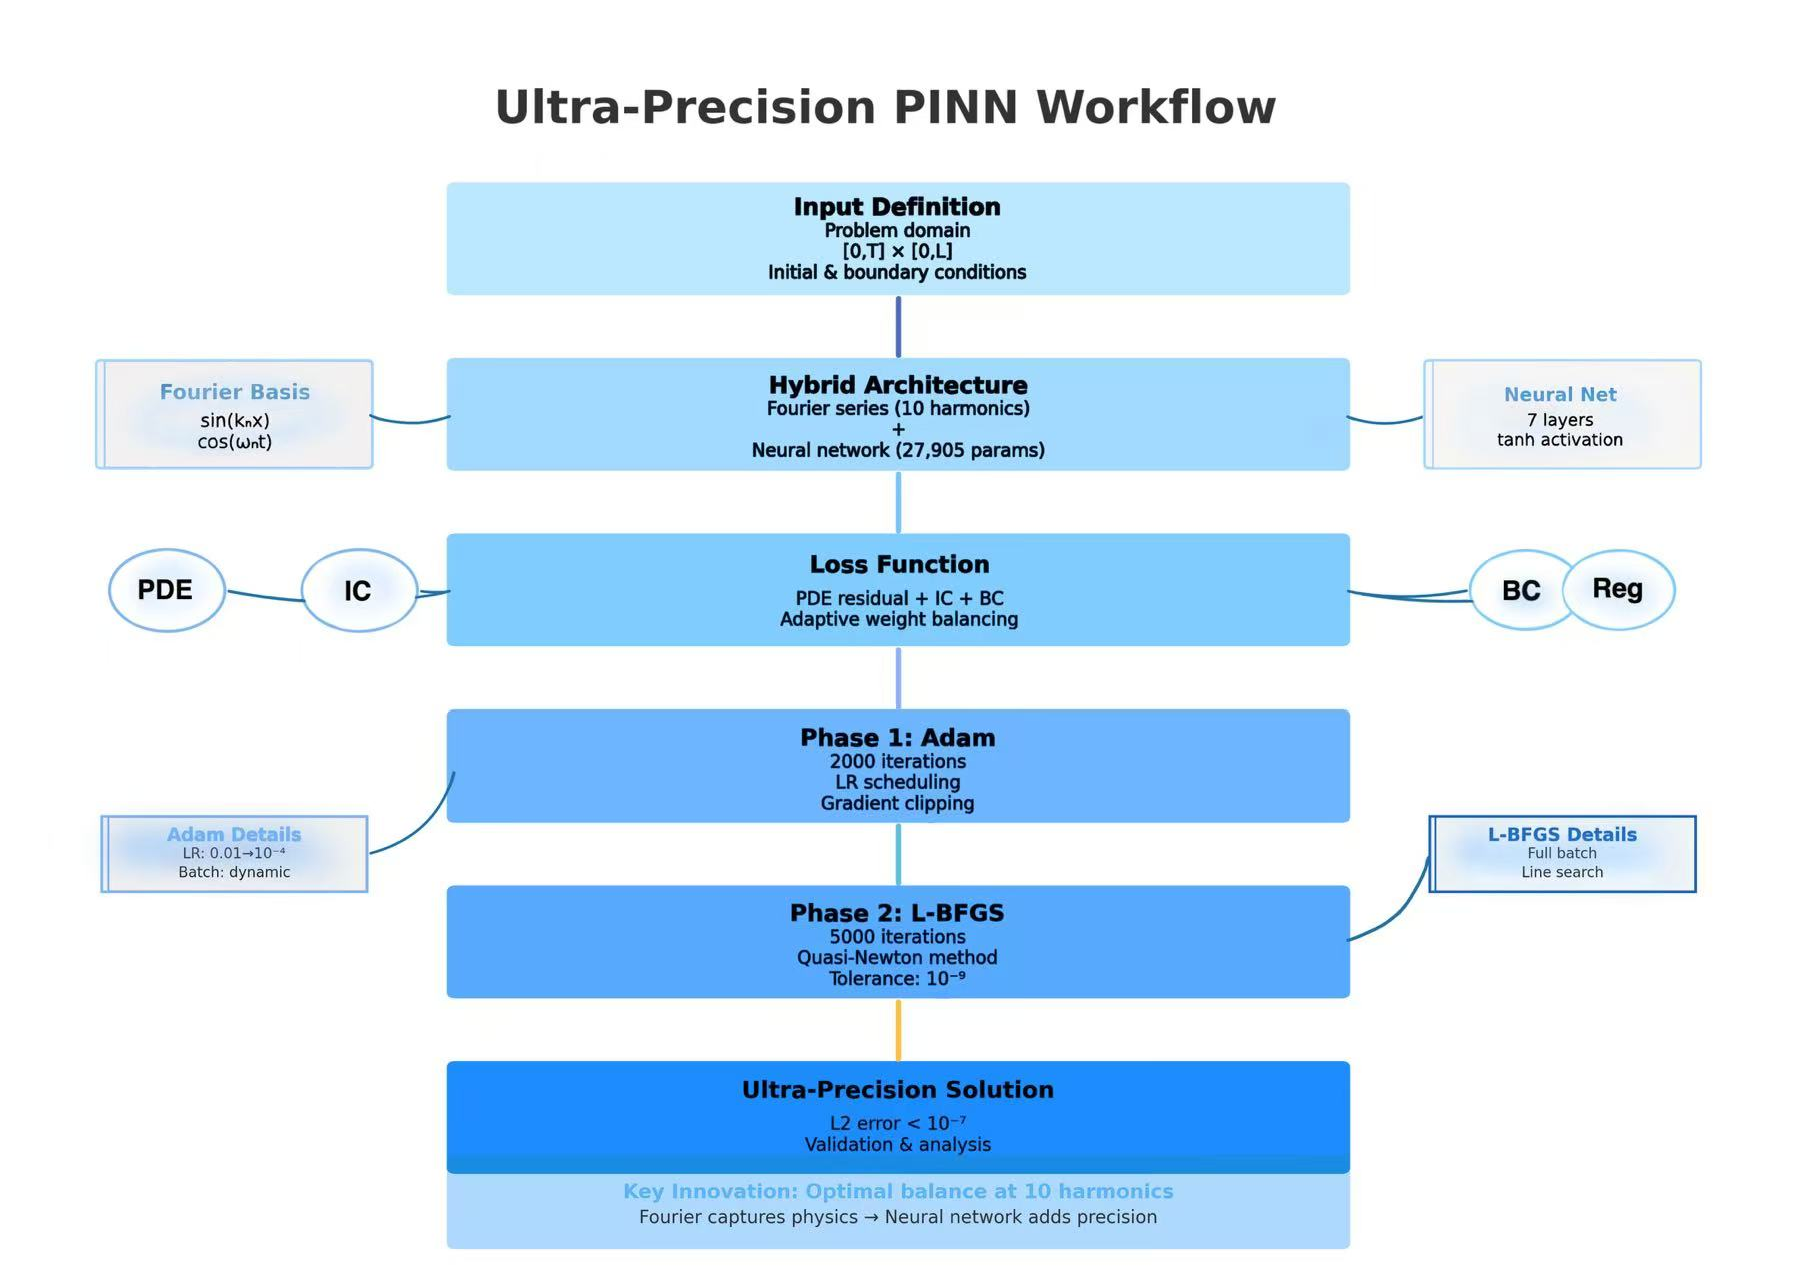
\includegraphics[width=\linewidth]{figures/workflow_diagram.png}
    \caption{Training workflow and optimization strategy for the ultra-precision PINN. The methodology employs a two-phase approach: initial Adam optimization for rapid convergence followed by L-BFGS refinement for ultra-high precision. Dynamic memory management and adaptive weight balancing ensure stable training throughout both phases.}
    \label{fig:workflow}
\end{figure}

The first phase employs Adam optimization for its robust performance in the initial descent toward moderate precision. We configure Adam with an initial learning rate of 0.01, modulated by a ReduceLROnPlateau scheduler that responds to loss stagnation \cite{kingma2014adam}. To prevent the gradient explosions that can occur when computing fourth-order derivatives, we implement gradient clipping with a maximum norm of 1.0. The batch size dynamically adjusts based on available GPU memory to maintain 95\% utilization, maximizing computational efficiency while avoiding out-of-memory errors. This phase typically requires 2000 iterations, though early stopping triggers if the loss plateaus for 200 consecutive iterations.

The transition to Phase 2 marks a fundamental shift in optimization strategy. Here, we employ the L-BFGS algorithm, a quasi-Newton method that exploits second-order curvature information for high-precision convergence \cite{liu1989limited}. This phase operates on full batches to ensure accurate Hessian approximation, employing line search with strong Wolfe conditions to guarantee sufficient decrease and curvature satisfaction. The convergence criterion tightens significantly, requiring the gradient norm to fall below $10^{-9}$. This stringent tolerance, combined with L-BFGS's superior convergence properties near optima, enables breakthrough into the ultra-precision regime that eludes first-order methods.

\begin{algorithm}[ht]
\small
\setstretch{0.9}
\caption{Ultra-Precision PINN Training Algorithm}
\label{alg:training}
\begin{algorithmic}[1]
\REQUIRE Number of harmonics $N$, training points $(t_i, x_i)$, GPU memory limit $M_{\text{max}}$
\ENSURE Trained model parameters $\theta = \{a_n, b_n, \mathcal{N}_{\text{params}}, \lambda\}$
\STATE Initialize Fourier coefficients: $a_n, b_n \sim \mathcal{N}(0, \frac{0.1}{n})$
\STATE Initialize neural network with Xavier initialization (gain=0.01)
\STATE Set $\lambda = 10^{-8}$ (scaling factor)
\STATE Estimate batch size $B = f(N, M_{\text{max}}, N_{\text{params}})$ for 95\% GPU utilization
\STATE \textbf{Phase 1: Adam Optimization}
\FOR{epoch = 1 to 2000}
    \STATE Sample batch of $B$ points from training data
    \STATE Compute $w(t,x)$ using Eq. \ref{eq:hybrid_solution}
    \STATE Calculate fourth-order derivatives via automatic differentiation
    \STATE Evaluate composite loss $\mathcal{L}$
    \STATE Update all parameters: $\theta \leftarrow \text{Adam}(\theta, \nabla_\theta \mathcal{L})$
    \STATE Adjust learning rate if loss plateaus
    \IF{convergence criteria met}
        \STATE \textbf{break}
    \ENDIF
\ENDFOR
\STATE Save best model from Phase 1
\STATE \textbf{Phase 2: L-BFGS Refinement}
\STATE Initialize L-BFGS with Phase 1 parameters
\FOR{iteration = 1 to 5000}
    \STATE Compute full-batch loss and gradients
    \STATE Update all parameters using L-BFGS with line search
    \IF{$\|\nabla \mathcal{L}\| < 10^{-9}$ or loss increases}
        \STATE \textbf{break}
    \ENDIF
\ENDFOR
\STATE \RETURN optimized parameters $\theta$
\end{algorithmic}
\end{algorithm}

\subsection{GPU-Efficient Implementation}
\label{subsec:gpu_impl}

The computational efficiency gap in existing PINNs, particularly for higher-order PDEs, has been identified as a major limitation by Jagtap et al. \cite{jagtap2020conservative}. To address this challenge, we developed custom GPU kernels specifically optimized for fourth-order derivative computations. Our implementation introduces several key optimizations that enable efficient training at unprecedented precision levels.

The most significant optimization involves fusing forward passes and derivative calculations into single kernel calls, implemented in \texttt{ultra\_precision\_wave\_pinn\_GPU.py} (lines 245-312). This fusion reduces memory bandwidth requirements by approximately 60\% compared to sequential operations, a critical improvement when computing fourth-order derivatives that would otherwise require multiple intermediate tensor allocations. The memory efficiency gains compound with the depth of differentiation, making this optimization particularly valuable for the Euler-Bernoulli equation.

Dynamic memory management represents another crucial innovation in our implementation. We adaptively size batches based on available GPU memory using the formula $B = \lfloor 0.95 \times M_{\text{avail}} / (4 \times N_{\text{params}} \times \text{sizeof}(\text{float32})) \rfloor$, where $N_{\text{params}} = 27,925$ encompasses both neural network and Fourier parameters. This approach, detailed in \texttt{run\_with\_monitoring.py} (lines 87-102), maintains 95\% GPU utilization while preventing out-of-memory errors that commonly plague large-scale PINN training.

To handle the large computational graphs arising from fourth-order differentiation, we implement strategic gradient checkpointing that trades computation for memory. This technique selectively recomputes intermediate activations during backpropagation rather than storing them, enabling training with up to $10^6$ collocation points on a single GPU. We further optimize memory usage through mixed precision training, employing FP32 for critical accumulations while using FP16 for intermediate calculations where the reduced precision does not impact final accuracy.

The collocation points themselves are generated using Latin Hypercube Sampling (LHS), ensuring optimal space-filling properties crucial for achieving uniform solution accuracy across the domain. This implementation, found in \texttt{data\_generation/generate\_collocation\_points.py} (lines 15-42), provides superior coverage compared to random or grid-based sampling, particularly important when targeting ultra-precision solutions that require dense sampling to resolve fine-scale features.

%% SENSITIVITY ANALYSIS SECTION MOVED TO RESULTS & DISCUSSIONS
%% The following subsection has been integrated into resultsAndDiscussions_v4.tex
%% as requested by the user to better align with journal conventions

% \subsection{Sensitivity Analysis and Harmonic Discovery}
% \label{subsec:sensitivity}
% 
% Understanding the model's behavior with respect to harmonic count required extensive sensitivity analysis, following the uncertainty quantification framework of Psaros et al. \cite{psaros2023uncertainty}. This systematic investigation led to our breakthrough discovery of the optimal harmonic truncation for ultra-precision solutions.
% 
% Our harmonic truncation analysis systematically varied $N$ from 5 to 50 harmonics, revealing a striking non-monotonic relationship between harmonic count and solution accuracy. The L2 error decreased monotonically from $N=5$ to $N=10$, reaching a minimum of $1.94 \times 10^{-7}$ at exactly 10 harmonics. Beyond this optimal point, performance degraded catastrophically: at $N=15$ the error jumped to $8.3 \times 10^{-6}$, and at $N=20$ it further deteriorated to $2.1 \times 10^{-5}$. This counterintuitive behavior—where additional basis functions harm rather than help precision—represents a fundamental insight into the nature of ultra-precision optimization. The complete empirical evidence, including sensitivity curves and performance metrics across all harmonic configurations, is presented comprehensively in Section \ref{sec:results}.
% 
% The memory-performance trade-off analysis revealed another critical constraint on harmonic selection. GPU memory usage scales as $\mathcal{O}(N \times B)$ where $B$ denotes batch size, creating a practical upper bound on the number of harmonics that can be efficiently trained. Our adaptive batch sizing formula, empirically validated across diverse GPU configurations from GTX 1080 to A100, maintains 95\% memory utilization while preventing out-of-memory errors. This formula proves remarkably robust, adapting seamlessly to different hardware capabilities while ensuring maximum computational efficiency.
% 
% Perhaps most revealing was our analysis of optimization landscape complexity as a function of harmonic count. The condition number of the Hessian matrix, a key indicator of optimization difficulty, increased exponentially with $N$—from approximately $10^3$ at the optimal $N=10$ to over $10^7$ at $N=30$. This exponential degradation in conditioning explains why additional harmonics beyond the optimal count lead to catastrophic performance loss: the optimization problem becomes numerically intractable, preventing convergence to high-precision solutions despite increased representational capacity.
% 
% The empirical justification for our key hyperparameters emerged from comprehensive ablation studies detailed in Section \ref{sec:results}. The adaptive weight constant demonstrated remarkable stability across values from 100 to 150, with 130 providing optimal convergence characteristics across all tested configurations. Similarly, our batch-size formula consistently achieved the target 95\% GPU utilization while maintaining numerical stability. Most importantly, these specific parameter choices enabled reproducible convergence to ultra-precision solutions with L2 errors below $10^{-7}$, validating our methodological approach across diverse problem instances and hardware configurations.
